%------------------------------------------------------------------------------
% Author(s):
% Varaun Ramgoolie
% Copyright:
%  Copyright (C) 2020 Brad Bachu, Arjun Mohammed, Nicholas Sammy, Kerry Singh
%
%  This file is part of Applied-Mathematics-Unit2 and is distributed under the
%  terms of the MIT License. See the LICENSE file for details.
%
%  Description:
%     Year: 2016
%     Module: 1
%     Question: 2 
%------------------------------------------------------------------------------
\usetikzlibrary{patterns}

\begin{subquestions}
	
%------------------------------------------------------------------------------
% 2 a--------------------------------------------------------------------------
%------------------------------------------------------------------------------

\subquestion

We must maximize the expression, $P=6x+4y$, given the following inequalities:

\begin{align}
	4x+6y & \leq 48\,, \nn \\
	4x+2y & \leq 32\,, \nn \\
	0 \leq & ~ y \leq 5\,, \nn \\
	x & \geq 0\,.
\end{align}

\begin{subsubquestions}

%------------------------------------------------------------------------------
% 2 a i------------------------------------------------------------------------
%------------------------------------------------------------------------------
	
\subsubquestion

See Graph ~\ref{2016:q2:graph:Graph1}.

\begin{figure}
	\centering
	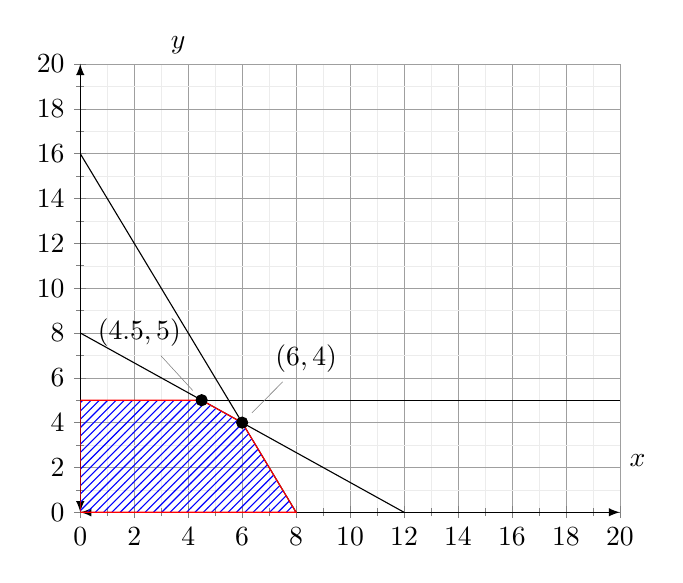
\begin{tikzpicture}
		\begin{axis}
			[
			xmin=-0,xmax=20,
			ymin=0,ymax=20,
			grid=both,
			grid style={line width=.1pt, draw=darkgray!10},
			major grid style={line width=.2pt,draw=darkgray!50},
			axis lines=left,
			minor tick num=1,
			enlargelimits={abs=0},
			axis line style={latex-latex},
			samples=100,
			domain = -20:20,
			ytick={0,2,4,...,20},
			xtick={0,2,4,...,20},
			xlabel={$x$},
			ylabel={$y$},
			x label style={at={(axis description cs:1,0.15)},anchor=north west},
			y label style={at={(axis description cs:0.15,1)},anchor=south west, rotate=-90}
			]
			
			\addplot [mark=dot] coordinates{(12,0)  (0,8)};
			
			\addplot [mark=dot] coordinates {(8,0) (0,16)};
			
			\addplot [mark=dot] coordinates {(0,5) (100,5)};
			
			\addplot [red,pattern=north east lines,pattern color=blue] coordinates {(0,5) (4.5,5) (6, 4) (8,0)} \closedcycle;	

			\node [pin=104:{$(4.5,5)$}] at (axis cs:4.5,5) {};

			\addplot [mark=*] coordinates{(4.5, 5)};

			\node [pin=60:{$(6,4)$}] at (axis cs:6,4) {};
			
			\addplot [mark=*] coordinates{(6,4)};
			
		\end{axis}
	\end{tikzpicture}
	\caption{\label{2016:q2:graph:Graph1} Graph showing the feasible region of the problem.} 
\end{figure}

%------------------------------------------------------------------------------
% 2 a ii------------------------------------------------------------------------
%------------------------------------------------------------------------------

\subsubquestion

The feasible region is shaded in Graph ~\ref{2016:q2:graph:Graph1}.

%------------------------------------------------------------------------------
% 2 a iii----------------------------------------------------------------------
%------------------------------------------------------------------------------

\subsubquestion

From ~\ref{mod1:defn:TourOfVertices}, we can calculate $P$ by,

\begin{align}
	\text{Using (0,5)} \,, \nn \\
	P & = 6x + 4y \,, \nn \\
      & = (6 \times 0) + (4 \times 5) \,, \nn \\
	  & = 20 \,. \\
	\text{Using (4.5,5)} \,, \nn \\
	P & = 6x + 4y \,, \nn \\
	  & = (6 \times 4.5) + (4 \times 5) \,, \nn \\
	  & = 47 \,.    \\		  
	\text{Using (6,4)} \,, \nn \\
	P & = 6x + 4y \,, \nn \\
	  & = (6 \times 6) + (4 \times 4) \,, \nn \\
	  & = 52 \,. \label{2016:q2:eqn:Profit} \\
	\text{Using (8,0)} \,, \nn \\
	P & = 6x + 4y \,, \nn \\
	  & = (6 \times 8) + (4 \times 0) \,, \nn \\
	  & = 48 \,. 
\end{align}

From \req{2016:q2:eqn:Profit}, we see that the maximum value of $P$ is 52.

\end{subsubquestions}

%------------------------------------------------------------------------------
% 2 b--------------------------------------------------------------------------
%------------------------------------------------------------------------------

\subquestion

\begin{subsubquestions}
	
\subsubquestion

The Hungarian algorithm is shown in \rtab{2016:q2:tab:HungAlgo}.

\begin{table}[!hbt]
	\begin{minipage}{0.3\textwidth}
		\centering
		\begin{tabular}{cccc}
			23 & 31 & 25 & 28 \\
			30 & 20 & 33 & 29 \\
			20 & 25 & 28 & 25 \\
			35 & 19 & 20 & 30 \\
		\end{tabular}
		\captionsetup{width=1.1\linewidth}
		\caption*{Matrix From question}
	\end{minipage}
	\hspace{20pt}
	%------------------------------------------------------------------------------
	\begin{minipage}{0.3\textwidth}
		\centering
		\begin{tabular}{cccc}
			0 & 8 & 2 & 5 \\
		   10 & 0 & 13 & 9 \\
			0 & 5 & 8 & 5 \\
		   16 & 0 & 1 & 11 \\
		\end{tabular}
		\captionsetup{width=1.1\linewidth}
		\caption*{Matrix after Reducing Rows}
	\end{minipage}
	\hspace{20pt}
	%------------------------------------------------------------------------------
	\begin{minipage}{0.3\textwidth}
		\centering
		\begin{tabular}{cccc}
			0 & 8 & 1 & 0 \\
		   10 & 0 & 12 & 4 \\
			0 & 5 & 7 & 0 \\
		   16 & 0 & 0 & 6 \\
		\end{tabular}
		\captionsetup{width=1.1\linewidth}
		\caption*{Matrix after Reducing Columns} 
	\end{minipage}
	
	\vspace{20pt} 
	%------------------------------------------------------------------------------
	\begin{minipage}{0.3\textwidth}
		\centering
		\begin{tabular} {cccccc}
			&   &        & 							 &   &                       \\ 
   \hhs{h1} & 0 &      8 &                         1 & 0 & \hhe[red]{h1}         \\
   \hhs{h2} &10 &      0 &                        12 & 4 & \hhe[red]{h2}         \\
   \hhs{h3}	& 0 &      5 &                         7 & 0 & \hhe[red]{h3}         \\
   \hhs{h4}	&16 &      0 &                         0 & 6 & \hhe[red]{h4}         \\
			&   &        & 							 &   &                       \\
		\end{tabular}
		\captionsetup{width=1.1\linewidth}
		\caption*{Shading 0's using the least \\ \centering number of lines}
	\end{minipage}
	\caption{\label{2016:q2:tab:HungAlgo} Showing the steps of the Hungarian Algorithm.}
\end{table}

From \rtab{2016:q2:tab:HungAlgo}, the possible matchings of the passengers and drivers are,

\begin{align}
	& A \rightarrow R,P \,, \nn \\
	& B \rightarrow H \,, \nn \\
	& C \rightarrow R,P \,, \nn \\
	& D \rightarrow H,S \,.
\end{align} 

Thus, the matchings that minimize the total travel time is,

\begin{align}
	& A \rightarrow R ~\text{or} ~P \,, \nn \\
	& B \rightarrow H \,, \nn \\
	& C \rightarrow R ~\text{or} ~P \,, \nn \\
	& D \rightarrow S \,.
\end{align} 

%------------------------------------------------------------------------------

\subsubquestion

Therefore, the minimum total travel time is,

\begin{equation}
	\text{Minimum Time} = 23+20+25+20 = 88\, \text{minutes}\,.
\end{equation}


\end{subsubquestions}

\end{subquestions}

